\subsubsection{Sorting}
\label{sec:optim:sort}

Traversing an irregular structure requires loading from memory the elements of the structure which, due to their irregular nature, can not be obtained in an optimized way through prefetching. Also, the elements of this structure which are consecutively accessed (especially in parallel) will most probably lie in distinct cache lines, hurting locality.

By changing the order of accesses in these structures, so that domain objects with similar traversal patterns become consecutive, temporal locality is improved as the elements a given object will touch are already likely to have been touched by the previous one.

Sorting these objects in applications where the domain refers to a notion of space can be performed using space-filling curves\footnote{A curve which touches every object in the domain only once. Examples of these curves are the Peano and Hilbert curves.} (for algorithms in the space domain like Barnes-hut). The examples described in this document use the CGAL library, implementing the traits required for spatial sorting in 3D.

\begin{figure}[!htp]
	\centering
	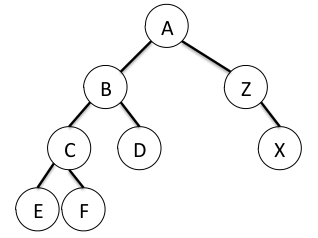
\includegraphics[width=0.4\columnwidth]{pointblocking_tree}
	\caption{A sample tree}
	\label{fig:tree}
\end{figure}

\begin{figure}[!htp]
	\centering
	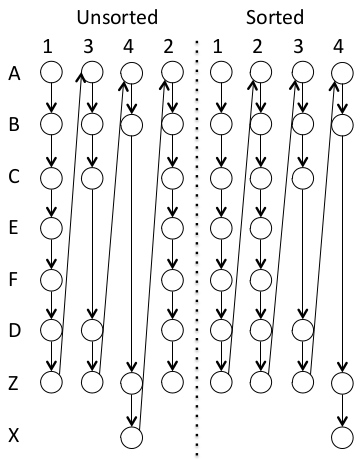
\includegraphics[width=0.6\columnwidth]{pointblocking_sort}
	\caption{Spatial Sort transformation applied to traversal of tree shown in \cref{fig:tree}}
	\label{fig:sort}
\end{figure}

\paragraph{Limitations:}
Processing objects in an order which brings similar traversals closer in time only brings improvements when the traversal itself fits in cache. This will allow subsequent objects to take advantage of the acceleration structure elements already visited by previous objects. For sufficiently deep traversals, when the subsequent objects traverse the structure, the first elements have already been evicted from cache. \cite{tree_tiler} already shows that as the traversal size increases, the locality improvements gained from the Sorting optimization decrease drastically.
